% Lecture Template for ME3001 - Mechanical Engineering Analysis - Tennessee Technological University
% Spring 2024 - condensing and streamlining lectures by combining topics into a single PDF under the module name
% this will simplify file and link management as well as make lectures easier to use in class
% - added image/ to clean directory and reduce redundancy, specific to module for now  

% Module Name: - Eigenvalues and Eigenvectors
% Topic 1 - Definition of Eigenvalue and Eigenvector 
% Topic 2 - 
% Topic 3 - 
% Topic 4 - 

\documentclass[fleqn]{beamer} % for presentation (has nav buttons at bottom)

\usepackage{../analysis_lectures}

\author{ME3001 - Mechanical Engineering Analysis}

\newcommand{\MNUM}{3\hspace{2mm}} % module number 
\newcommand{\moduletitle}{Eigenvalues and Eigenvectors}

\newcommand{\sectionItitle}{Definition of Eigenvalue and Eigenvector}
\newcommand{\sectionIItitle}{Engineering Applications}
\newcommand{\sectionIIItitle}{}
\newcommand{\sectionIVtitle}{}

\newcommand{\sectionIsubsectionItitle}{Mathematical Definition of Eigenvalue and Eigenvector}
\newcommand{\sectionIsubsectionIItitle}{Standard Eigenvalue Problem}
\newcommand{\sectionIsubsectionIIItitle}{The Geometrical Explanation}
\newcommand{\sectionIsubsectionIVtitle}{A Simple Example by Hand}

\newcommand{\sectionIIsubsectionItitle}{Forms of Standard Eigenvalue Problem}
\newcommand{\sectionIIsubsectionIItitle}{Solvability of Eigenvalue Problem}
\newcommand{\sectionIIsubsectionIIItitle}{Application 1 - Forging Hammer}
\newcommand{\sectionIIsubsectionIVtitle}{Application 2 - Principal Stress}
\newcommand{\sectionIIsubsectionVtitle}{Examples}

\newcommand{\sectionIIIsubsectionItitle}{}
\newcommand{\sectionIIIsubsectionIItitle}{}
\newcommand{\sectionIIIsubsectionIIItitle}{}
\newcommand{\sectionIIIsubsectionIVtitle}{}

\newcommand{\sectionIVsubsectionItitle}{}
\newcommand{\sectionIVsubsectionIItitle}{}
\newcommand{\sectionIVsubsectionIIItitle}{}
\newcommand{\sectionIVsubsectionIVtitle}{}

% custom box
\newsavebox{\mybox}

\title{Lecture Module - \moduletitle}

\date{Mechanical Engineering\vspc Tennessee Technological University}

\begin{document}

	\lstset{language=MATLAB,basicstyle=\ttfamily\small,showstringspaces=false}

	\frame{\titlepage \center\begin{framed}\Large \textbf{Module \MNUM - \moduletitle}\end{framed} \vspace{5mm}}

	% Module Outline
	\begin{frame} 
		\large \textbf{Module \MNUM - \moduletitle} \vspace{3mm}\\

		\begin{itemize}
			\item Topic 1 - \hyperlink{sectionI}{\sectionItitle} \vspc % section I
			\item Topic 2 - \hyperlink{sectionII}{\sectionIItitle} \vspc % section II
			\item Topic 3 - \hyperlink{sectionIII}{\sectionIIItitle} \vspc % section III
		\end{itemize}

	\end{frame}

	% section I
	\section{\sectionItitle}\label{sectionI}

		% section I Outline
		\begin{frame} 
			\large \textbf{Topic 1 - \sectionItitle} \vspace{3mm}\\

			\begin{itemize}
				\item \hyperlink{sectionIsubsectionI}{\sectionIsubsectionItitle} \vspc %  section I subsection I
				\item \hyperlink{sectionIsubsectionII}{\sectionIsubsectionIItitle} \vspc % section I subsection II
				\item \hyperlink{sectionIsubsectionIII}{\sectionIsubsectionIIItitle} \vspc % section I subsection III
				\item \hyperlink{sectionIsubsectionIV}{\sectionIsubsectionIVtitle} \vspc % section I subsection IV
			\end{itemize}
		\end{frame}
		
		% section I subsection I 
		\subsection{\sectionIsubsectionItitle}\label{sectionIsubsectionI}

			\begin{frame}
				\frametitle{\sectionIsubsectionItitle}
				\bigskip

				\textbf{Did you study this in calculus? Differential Equations?} \vspace{3mm}

				In linear algebra, an eigenvector or characteristic vector of a linear transformation is a non-zero vector whose direction does not change when that linear transformation is applied to it. More formally, if $T$ is a linear transformation from a vector space $V$ over a field $F$ into itself and $v$ is a vector in $V$ that is not the zero vector, then $v$ is an eigenvector of $T$ if $T(v)$ is a scalar multiple of $v$. This condition can be written as the equation\\

				\[ T({\bf v})=\lambda{\bf v} \]


				\btVFill
			\end{frame}

			\begin{frame}
				\frametitle{\sectionIsubsectionItitle}
				\bigskip

				where $\lambda$ is a scalar in the field $F$, known as the eigenvalue, characteristic value, or characteristic root associated with the eigenvector $v$.

				If the vector space $V$ is finite-dimensional, then the linear transformation $T$ can be represented as a square matrix $A$, and the vector $v$ by a column vector, rendering the above mapping as a matrix multiplication on the left hand side and a scaling of the column vector on the right hand side in the equation.\\

				\[ [A]{\bf v}=\lambda{\bf v} \]

				\btVFill
			\end{frame}

		% section I subsection II
		\subsection{\sectionIsubsectionIItitle}\label{sectionIsubsectionII}

			\begin{frame}
				\frametitle{\sectionIsubsectionIItitle} \small
				\bigskip

				\scalebox{1.0}{\parbox{.5\linewidth}{
				\[ \left( \begin{array}{cccc}
				a_{11}  & a_{12} & ...& a_{1n} \\
				a_{21} & a_{22}  & ...& a_{2n} \\
				&.&&\\
				&.&&\\
				a_{n1} & a_{n2} & ...& a_{nn} \end{array} \right) \times \left[ \begin{array}{c}
				x_1 \\
				x_2 \\
				.\\
				.\\
				x_n \end{array} \right] = \lambda\left[ \begin{array}{c}
				x_1 \\
				x_2 \\
				.\\
				.\\
				x_n \end{array} \right]\] 
				}}
	  	 		
	  	 		\scalebox{1.0}{\parbox{.5\linewidth}{
				\[ \left(\left[ \begin{array}{cccc}
				a_{11}  & a_{12} & ...& a_{1n} \\
				a_{21} & a_{22}  & ...& a_{2n} \\
				&.&&\\
				&.&&\\
				a_{n1} & a_{n2} & ...& a_{nn} \end{array} \right]-\lambda\left[ \begin{array}{cccc}
				1  & 0 & ...& 0 \\
				0 & 1  & ...& 0 \\
				0 & 0  & 1 & 0 \\
				&.&&\\
				0 & 0 & ...& 1 \end{array} \right]\right) \times \left[ \begin{array}{c}
				x_1 \\
				x_2 \\
				.\\
				.\\
				x_n \end{array} \right] = \left[ \begin{array}{c}
				0\\
				0 \\
				.\\
				.\\
				0 \end{array} \right]\] 
				}}

				\btVFill
			\end{frame}


			\begin{frame}
				\frametitle{\sectionIsubsectionIItitle} \small
				\bigskip

				The Equations \vspace{1mm}\\
				\[(a_{11}-\lambda) x_1 + a_{12} x_{2} + ... + a_{1n} x_n = 0 \]
				\[a_{21} x_1 + (a_{22}-\lambda)  x_{2} + ... + a_{2n} x_n = 0 \]
				\[. . .\]
				\[. . .\]
				\[a_{n1} x_1 + a_{n2} x_{2} + ... + (a_{nn}-\lambda) x_n = 0 \]	

				The Matrix Form \\
				%\begin{fleqn}
				\scalebox{1.0}{\parbox{.5\linewidth}{
				\[ \left( \begin{array}{cccc}
				(a_{11}-\lambda)  & a_{12} & ...& a_{1n} \\
				a_{21} & (a_{22}-\lambda)  & ...& a_{2n} \\
				&. . .&&\\
				&. . .&&\\
				a_{n1} & a_{n2} & ...& (a_{nn}-\lambda) \end{array} \right) \times \left[ \begin{array}{c}
				x_1 \\
				x_2 \\
				. \\
				. \\
				x_n \end{array} \right] = \left[ \begin{array}{c}
				0 \\
				0 \\
				. \\
				. \\
				0 \end{array} \right]\] 
				}}		
				%\end{fleqn}

				\btVFill
			\end{frame}

		% section I subsection III
		\subsection{\sectionIsubsectionIIItitle}\label{sectionIsubsectionIII}
			\begin{frame} 
				\frametitle{\sectionIsubsectionIIItitle} \small
				\bigskip

				\textbf{Look at the second matrix form closely}\\

				\[ ([A]-\lambda[I])\{x\}=\{0\} \]

				First we need to realize that this matrix system is {\it Homogeneous}. This follows a different rule regarding the existence of a solution.\\
				 A {\it Homogeneous} system has a non-trivial solution if and only if the determinant of the coefficient matrix is zero.\\

				\[ |[A]|=0 \]

				Therefore the following must be true\\
				\[ |[A]-\lambda[I]|=0 \]

				This leads to a long $n^{th}$ order polynomial in terms of $\lambda$. This will have $n$ roots which may be real or complex.

				\btVFill
			\end{frame}	

			\begin{frame} 
				\frametitle{\sectionIsubsectionIIItitle}
				\bigskip

				3x3 example \\
				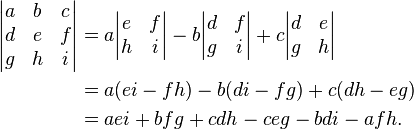
\includegraphics[scale=.5]{images/lecture5_fig1.png}
	
				\btVFill
			\end{frame}	

			\begin{frame} 
				\frametitle{\sectionIsubsectionIIItitle}
				\bigskip


				\btVFill
			\end{frame}	

			\begin{frame} 
				\frametitle{\sectionIsubsectionIIItitle}
				\bigskip
	
				
				\btVFill
			\end{frame}	


		% section I subsection IV
		\subsection{\sectionIsubsectionIVtitle}\label{sectionIsubsectionIV}	

			\begin{frame}
				\frametitle{\sectionIsubsectionIVtitle}
				\bigskip


				\btVFill
			\end{frame}
	
	% Section II
	\section{\sectionIItitle}\label{sectionII}

		% section II Outline
		\begin{frame}
			\large \textbf{Topic 2 - \sectionIItitle} \vspace{3mm}\\

			\begin{itemize}
				\item \hyperlink{sectionIIsubsectionI}{\sectionIIsubsectionItitle} \vspc %  section II subsection I
				\item \hyperlink{sectionIIsubsectionII}{\sectionIIsubsectionIItitle} \vspc % section II subsection II
				\item \hyperlink{sectionIIsubsectionIII}{\sectionIIsubsectionIIItitle} \vspc % section II subsection III
				\item \hyperlink{sectionIIsubsectionIV}{\sectionIIsubsectionIVtitle} \vspc % section II 
			\end{itemize}

			This section was written by Mike Renfro and/or others.

		\end{frame}

		% section II subsection I
		\subsection{\sectionIIsubsectionItitle}\label{sectionIIsubsectionI}

			\begin{frame}[label=sectionIIsubsectionI]
				\frametitle{\sectionIIsubsectionItitle} \small
				\bigskip

				 Consider a system of equations in algebraic form
  \begin{align*}
    (a_{11}-\lambda) x_1 + a_{12} x_2 + a_{13} x_3 + \cdots + a_{1n} x_n =& 0 \\
    a_{21} x_1 + (a_{22}-\lambda) x_2 + a_{23} x_3 + \cdots + a_{2n} x_n =& 0 \\
    \vdots{}& \\
    a_{n1} x_1 + a_{n2} x_2 + a_{n3} x_3 + \cdots + (a_{nn}-\lambda) x_n =& 0 \\
  \end{align*}
  This is not a normal system of linear algebraic equations we're used
  to. For one, there are $n$ equations, but $n+1$ unknowns (the $x_i$
  values, and also $\lambda$). This particular system of equations is
  known as \emph{the standard eigenvalue problem}.


				\btVFill
			\end{frame}

			\begin{frame}[label=sectionIIsubsectionI]
				\frametitle{\sectionIIsubsectionItitle} \small
				\bigskip

 The three forms shown are all algebraically equivalent. Any system
  of equations that can be expressed in these forms is a standard
  eigenvalue problem.

  \begin{displaymath}
    \left[ \begin{array}{cccc}
        a_{11}-\lambda & a_{12} & \cdots & a_{1n} \\
        a_{21} & a_{22}-\lambda & \cdots & a_{2n} \\
        \vdots & \vdots & \ddots & \vdots \\
        a_{n1} & a_{n2} & \cdots & a_{nn}-\lambda
      \end{array} \right]
    \left\{ \begin{array}{c}
        x_1 \\
        x_2 \\
        \vdots \\
        x_n
      \end{array} \right\} =
    \left\{ \begin{array}{c}
        0 \\
        0 \\
        \vdots \\
        0
      \end{array} \right\}
  \end{displaymath}				

			
				\btVFill
			\end{frame}	

			\begin{frame}[label=sectionIIsubsectionI]
				\frametitle{\sectionIIsubsectionItitle} \small
				\bigskip

 \frametitle{Form 2}
  \begin{displaymath}
    \left( \left[ \begin{array}{cccc}
          a_{11} & a_{12} & \cdots & a_{1n} \\
          a_{21} & a_{22} & \cdots & a_{2n} \\
          \vdots & \vdots & \ddots & \vdots \\
          a_{n1} & a_{n2} & \cdots & a_{nn}
        \end{array} \right] -
      \lambda \left[ \begin{array}{cccc}
          1 & 0 & \cdots & 0 \\
          0 & 1 & \cdots & 0 \\
          \vdots & \vdots & \ddots & \vdots \\
          0 & 0 & \cdots & 1
        \end{array} \right] \right)
    \left\{ \begin{array}{c}
        x_1 \\
        x_2 \\
        \vdots \\
        x_n
      \end{array} \right\} =
    \left\{ \begin{array}{c}
        0 \\
        0 \\
        \vdots \\
        0
      \end{array} \right\}
  \end{displaymath}
  \begin{displaymath}
    \left( \left[A\right] - \lambda \left[ I \right] \right) \left\{ x \right\} = \left\{ 0 \right\}
  \end{displaymath}

				
				\btVFill
			\end{frame}

		\begin{frame}[label=sectionIIsubsectionI]
				\frametitle{\sectionIIsubsectionItitle}
				\bigskip

				 \frametitle{Form 3}
  \begin{displaymath}
    \left[ \begin{array}{cccc}
        a_{11} & a_{12} & \cdots & a_{1n} \\
        a_{21} & a_{22} & \cdots & a_{2n} \\
        \vdots & \vdots & \ddots & \vdots \\
        a_{n1} & a_{n2} & \cdots & a_{nn}
      \end{array} \right]
    \left\{ \begin{array}{c}
        x_1 \\
        x_2 \\
        \vdots \\
        x_n
      \end{array} \right\} =
    \lambda
    \left\{ \begin{array}{c}
        x_1 \\
        x_2 \\
        \vdots \\
        x_n
      \end{array} \right\}
  \end{displaymath}
  \begin{displaymath}
    \left[ A \right] \left\{ x \right\} = \lambda \left\{ x \right\}
  \end{displaymath}
			
				\btVFill
			\end{frame}

		% section II subsection II
		\subsection{\sectionIIsubsectionIItitle}\label{sectionIIsubsectionII}

			\begin{frame}
				\frametitle{\sectionIIsubsectionIItitle} \small
				\bigskip

				  \frametitle{Solvability of the Standard Eigenvalue Problem}
				  Recall form 2 of the standard eigenvalue problem:
				  \begin{displaymath}
				    \left( \left[A\right] - \lambda \left[ I \right] \right) \left\{ x \right\} = \left\{ 0 \right\}
				  \end{displaymath}
				  This system of equations has a solution for values of $\lambda$ that
				  cause the determinant of the coefficient matrix to equal 0, that is:
				  \begin{displaymath}
				    \left| \left[ A \right] - \lambda \left[ I \right] \right| = 0
				  \end{displaymath}

				\btVFill 
			\end{frame}	

			\begin{frame}
				\frametitle{\sectionIIsubsectionIItitle} \small
				\bigskip

				 \frametitle{Characteristic Equation}
  
				  Expanding out all the terms of the previous determinant
				  \begin{displaymath}
				    \left| \begin{array}{cccc}
				        a_{11}-\lambda & a_{12} & \cdots & a_{1n} \\
				        a_{21} & a_{22}-\lambda & \cdots & a_{2n} \\
				        \vdots & \vdots & \ddots & \vdots \\
				        a_{n1} & a_{n2} & \cdots & a_{nn}-\lambda
				      \end{array} \right| = 0
				  \end{displaymath}
				  yields a long polynomial in terms of $\lambda$. This polynomial will
				  be $n$th order, and will therefore have $n$ roots, each of which may
				  be real or complex.

				\btVFill
			\end{frame}		


		% section II subsection III
		\subsection{\sectionIIsubsectionIIItitle}\label{sectionIIsubsectionIII}

			\begin{frame}
				\frametitle{\sectionIIsubsectionIIItitle} \small
				\bigskip

				\frametitle{General Eigenvalue Problem: Introduction}
  
				Many physical systems do not automatically present themselves as a
				standard eigenvalue problem, even though they can be reformatted as
				a standard eigenvalue problem. The form of a \emph{general
				eigenvalue problem} is
				\begin{displaymath}
				\left[ A \right] \left\{ x \right\} = \lambda \left[ B \right] \left\{ x \right\}
				\end{displaymath}
				where $[A]$ and $[B]$ are symmetric matrices of size $n \times n$.
							
				\btVFill 
			\end{frame}

			\begin{frame}
				\frametitle{\sectionIIsubsectionIIItitle}\small
				\bigskip

				\frametitle{General Eigenvalue Problem Example}
				\begin{columns}
					\begin{column}{0.5\textwidth}
						A forging hammer of mass $m_2$ is mounted on a concrete
						foundation block of mass $m_1$. The stiffnesses of the springs
						underneath the forging hammer and the foundation block are given
						by $k_2$ and $k_1$, respectively.
					\end{column}
					\begin{column}{0.5\textwidth}
						\pgfimage[width=0.9\textwidth]{images/fig41a}
					\end{column}
				\end{columns}

				\btVFill 
			\end{frame}

			\begin{frame}
				\frametitle{\sectionIIsubsectionIIItitle}\small
				\bigskip

				 \frametitle{General Eigenvalue Problem Example}

				  \begin{columns}
				    \begin{column}{0.5\textwidth}
				      The system undergoes simple harmonic motion at one of its
				      natural frequencies $\omega$. That is:
				      \begin{displaymath}
				        x_1(t) = \cos ( \omega t + \phi_1 )
				      \end{displaymath}
				      \begin{displaymath}
				        x_2(t) = \cos ( \omega t + \phi_2 )
				      \end{displaymath}
				      \begin{displaymath}
				        a_1(t) = - \omega^2 x_1(t)
				      \end{displaymath}
				      \begin{displaymath}
				        a_2(t) = - \omega^2 x_2(t)
				      \end{displaymath}
				    \end{column}
				    \begin{column}{0.5\textwidth}
				      \pgfimage[width=0.9\textwidth]{images/fig41a}
				    \end{column}
				  \end{columns}

				\btVFill 
			\end{frame}

			\begin{frame}
				\frametitle{\sectionIIsubsectionIIItitle}\small
				\bigskip

				  \frametitle{General Eigenvalue Problem Example}

				  \begin{columns}
				    \begin{column}{0.7\textwidth}
				      Each mass in the system obeys Newton's second law of motion,
				      that is:
				      \begin{displaymath}
				        \Sigma F = m a
				      \end{displaymath}
				      Forces on the foundation block:
				      \begin{itemize}
				      \item forces from the lower springs, which counteracts motion in
				        the $x$ direction at an amount $-k_1 x_1$
				      \item forces from the upper springs, which act according to the
				        amount of relative displacement of the masses $m_1$ and $m_2$:
				        $-k_2 (x_1 - x_2)$
				      \end{itemize}
				    \end{column}
				    \begin{column}{0.3\textwidth}
				      \pgfimage[width=0.9\textwidth]{images/fig41b}
				    \end{column}
				  \end{columns}

				\btVFill 
			\end{frame}

			\begin{frame}
				\frametitle{\sectionIIsubsectionIIItitle}\small
				\bigskip

				  \frametitle{General Eigenvalue Problem Example}

				  \begin{columns}
				    \begin{column}{0.7\textwidth}
				      The equilibrium equation for the foundation mass is then
				      \begin{align*}
				        \Sigma F &= m a \\
				        -k_1 x_1 -k_2 (x_1 - x_2) &= m_1 a \\
				        (-k_2 - k_1) x_1 + k_2 x_2 &= m_1 a \\
				        (-k_2 - k_1) x_1 + k_2 x_2 &= -m_1 \omega^2 x_1 \\
				        (k_1 + k_2) x_1 - k_2 x_2 &= m_1 \omega^2 x_1
				      \end{align*}
				    \end{column}
				    \begin{column}{0.3\textwidth}
				      \pgfimage[width=0.9\textwidth]{images/fig41b}
				    \end{column}
				  \end{columns}

				\btVFill 
			\end{frame}

			\begin{frame}
				\frametitle{\sectionIIsubsectionIIItitle}\small
				\bigskip

				  \frametitle{General Eigenvalue Problem Example}
				  \begin{columns}
				    \begin{column}{0.7\textwidth}
				      Similarly, the equilibrium equation for the forging hammer mass
				      is
				      \begin{align*}
				        -k_2 x_1 + k_2 x_2 &= m_2 \omega^2 x_2
				      \end{align*}
				    \end{column}
				    \begin{column}{0.3\textwidth}
				      \pgfimage[width=0.9\textwidth]{images/fig41b}
				    \end{column}
				  \end{columns}

				\btVFill 
			\end{frame}

			\begin{frame}
				\frametitle{\sectionIIsubsectionIIItitle}\small
				\bigskip

				  \frametitle{General Eigenvalue Problem Example}

				  So the two equations of motion are
				  \begin{align*}
				    (k_1 + k_2) x_1 - k_2 x_2 &= m_1 \omega^2 x_1 \\
				    -k_2 x_1 + k_2 x_2 &= m_2 \omega^2 x_2
				  \end{align*}
				  or in matrix form
				  \begin{displaymath}
				    \left[ \begin{array}{cc}
				        k_1 + k_2 & -k_2 \\
				        -k_2 & k_2
				      \end{array} \right]
				    \left\{ \begin{array}{c}
				        x_1 \\
				        x_2
				      \end{array} \right\} =
				    \omega^2
				    \left[ \begin{array}{cc}
				        m_1 & 0 \\
				        0 & m_2
				      \end{array} \right]
				    \left\{ \begin{array}{c}
				        x_1 \\
				        x_2
				    \end{array} \right\}
				  \end{displaymath}
				  
				  This is a general eigenvalue problem
				  \begin{displaymath}
				    [A]\{x\} = \lambda [B] \{x\}
				  \end{displaymath}
				  where $[A]$ is the spring matrix, $\{x\}$ is the vector of $x$
				  values, $\lambda$ is $\omega^2$, and $[B]$ is the mass matrix.

				\btVFill 
			\end{frame}


		% section II subsection IV 
		\subsection{\sectionIIsubsectionIVtitle}\label{sectionIIsubsectionIV}

			\begin{frame}
				\frametitle{\sectionIIsubsectionIVtitle}
				\bigskip

				\frametitle{Eigenvalue Solutions in MATLAB: Standard Problems}
  
				  The design of a mechanical component requires that the maximum
				  principal stress to be less than the material strength. For a
				  component subjected to arbitrary loads, the principal stresses
				  $\sigma$ are given by the solution of the equation
				  \begin{displaymath}
				    \left[ \begin{array}{ccc}
				        \sigma_{xx} & \tau_{xy} & \tau_{xz} \\
				        \tau_{xy} & \sigma_{yy} & \tau_{yz} \\
				        \tau_{xz} & \tau_{yz} & \sigma_{zz}
				    \end{array} \right]
				    \left\{ \begin{array}{c}
				        l_x \\
				        l_y \\
				        l_z
				      \end{array} \right\} =
				    \sigma
				    \left\{ \begin{array}{c}
				        l_x \\
				        l_y \\
				        l_z
				      \end{array} \right\}
				  \end{displaymath}
				  where the $\sigma$ values represent normal stresses in the $x$, $y$,
				  and $z$ directions, and the $\tau$ values represent shear stresses
				  in the $xy$, $xz$, and $yz$ planes. The $l$ values represent
				  direction cosines that define the principal planes on which the
				  principal stress occurs.

				\btVFill 
			\end{frame}

			\begin{frame}
				\frametitle{\sectionIIsubsectionIVtitle}
				\bigskip

				 \frametitle{Eigenvalue Solutions in MATLAB: Standard Problems}
				  \begin{columns}
				    \begin{column}{0.7\textwidth}
				      Determine the principal stresses and principal planes in a
				      machine component for the following stress condition
				      \begin{displaymath}
				        \left[ \begin{array}{ccc}
				            \sigma_{xx} & \tau_{xy} & \tau_{xz} \\
				            \tau_{xy} & \sigma_{yy} & \tau_{yz} \\
				            \tau_{xz} & \tau_{yz} & \sigma_{zz}
				          \end{array} \right] =
				        \left[ \begin{array}{rrr}
				            10 & 4 & -6 \\
				            4 & -6 & 8 \\
				            -6 & 8 & 14
				          \end{array} \right] \text{~MPa}
				      \end{displaymath}
				    \end{column}
				    \begin{column}{0.3\textwidth}
				      \pgfimage[width=0.9\textwidth]{images/fig413}
				    \end{column}
				  \end{columns}

				\btVFill 
			\end{frame}
		
			\begin{frame}[fragile]
				\frametitle{\sectionIIsubsectionIVtitle}
				\bigskip

				 \frametitle{MATLAB Solution}
				  \begin{lstlisting}
				clear all
				sigma=[10  4 -6
				        4 -6  8
				       -6  8 14];
				[dirs,stresses]=eig(sigma);
				% diag(A) extracts the elements of the
				% [A] matrix along the diagonal
				principalStressList=diag(stresses)
				principalDirs=dirs
				  \end{lstlisting}

				\btVFill 
			\end{frame}

			\begin{frame}[fragile]
				\frametitle{\sectionIIsubsectionIVtitle}
				\bigskip

				  \frametitle{MATLAB Solution}
			  \begin{lstlisting}
			>> rao_p431
			principalStressList =
			  -10.4828
			    9.3181
			   19.1647
			principalDirs =
			   -0.2792    0.8343   -0.4754
			    0.8905    0.4102    0.1970
			   -0.3594    0.3683    0.8574
			  \end{lstlisting}


				\btVFill 
			\end{frame}

		
		% section II subsection V 
		\subsection{\sectionIIsubsectionVtitle}\label{sectionIIsubsectionV}	

			\begin{frame}
				\frametitle{\sectionIIsubsectionVtitle}
				\bigskip

				\frametitle{Eigenvalue Solutions in MATLAB: General Problems}
			  \begin{columns}
			    \begin{column}{0.5\textwidth}
			      Solve the forging hammer problem for the following values:
			      \begin{itemize}
			      \item $m_1 = 20000 \text{~kg}$
			      \item $m_2 = 5000 \text{~kg}$
			      \item $k_1 = 1 \times 10^7 \text{~N/m}$
			      \item $k_2 = 5 \times 10^6 \text{~N/m}$
			      \end{itemize}
			    \end{column}
			    \begin{column}{0.5\textwidth}
			      \pgfimage[width=0.9\textwidth]{images/fig41a}
			    \end{column}
			  \end{columns}

				\btVFill 
			\end{frame}


			\begin{frame}
				\frametitle{\sectionIIsubsectionVtitle}
				\bigskip

				  \frametitle{Solving Eigenvalue Problems in MATLAB}
  
				  Solving this eigenvalue problem will yield 2 eigenvalues equal to
				  the square of the system's natural frequencies, and 2 corresponding
				  $x$ vector values that show the relative displacements of the $m_1$
				  and $m_2$ masses at those frequencies.

				\btVFill 
			\end{frame}



			\begin{frame}[fragile]
				\frametitle{\sectionIIsubsectionVtitle}
				\bigskip

				  \frametitle{MATLAB Solution (Part 1)}

				  \begin{lstlisting}
				clear all;
				% Define spring constants and masses
				% for hammer and foundation block
				k1=1e7;
				k2=5e6;
				m1=20000;
				m2=5000;

				% Define system stiffness matrix
				K=[k1+k2 -k2
				     -k2  k2];
				% Define system mass matrix
				M=[m1  0
				    0 m2];
				  \end{lstlisting}


				\btVFill 
			\end{frame}



			\begin{frame}[fragile]
				\frametitle{\sectionIIsubsectionVtitle}
				\bigskip

				  \frametitle{MATLAB Solution (Part 2)}

			  \begin{lstlisting}
			% Solve general eigenvalue problem
			[X,Omega2]=eig(K,M);
			% diag(A) extracts the elements of the
			% [A] matrix along the diagonal
			Omega=diag(sqrt(Omega2));
			% Scale column 1 of the [X] matrix by
			% the row 1, column 1 X value
			X(:,1)=X(:,1)/X(1,1);
			% Scale column 2 of the [X] matrix by
			% the row 1, column 2 X value
			X(:,2)=X(:,2)/X(1,2);

			Omega
			X
			  \end{lstlisting}


				\btVFill 
			\end{frame}


			\begin{frame}[fragile]
				\frametitle{\sectionIIsubsectionVtitle}
				\bigskip

				  \frametitle{MATLAB Solution (Part 2)}

			  \begin{lstlisting}
			% Solve general eigenvalue problem
			[X,Omega2]=eig(K,M);
			% diag(A) extracts the elements of the
			% [A] matrix along the diagonal
			Omega=diag(sqrt(Omega2));
			% Scale column 1 of the [X] matrix by
			% the row 1, column 1 X value
			X(:,1)=X(:,1)/X(1,1);
			% Scale column 2 of the [X] matrix by
			% the row 1, column 2 X value
			X(:,2)=X(:,2)/X(1,2);

			Omega
			X
			  \end{lstlisting}


				\btVFill 
			\end{frame}


			\begin{frame}[fragile]
				\frametitle{\sectionIIsubsectionVtitle}
				\bigskip

				  \frametitle{MATLAB Solution (Results)}

				  \begin{lstlisting}
				>> rao_ex42
				Omega =
				   18.9634
				   37.2879
				X =
				    1.0000    1.0000
				    1.5616   -2.5616
				  \end{lstlisting}

				\btVFill 
			\end{frame}


	% section III and IV not used for now		
	% Section III
	% \section{\sectionIIItitle}\label{sectionIII}

	% 	% section III Outline
	% 	\begin{frame}
	% 		\large \textbf{Topic 3 - \sectionIIItitle} \vspace{3mm}\\

	% 		\begin{itemize}
	% 			\item \hyperlink{sectionIIIsubsectionI}{\sectionIIIsubsectionItitle} \vspc %  section III subsection I
	% 			\item \hyperlink{sectionIIIsubsectionII}{\sectionIIIsubsectionIItitle} \vspc % section III subsection II
	% 			\item \hyperlink{sectionIIIsubsectionIII}{\sectionIIIsubsectionIIItitle} \vspc % section III subsection III
	% 			\item \hyperlink{sectionIIIsubsectionIV}{\sectionIIIsubsectionIVtitle} \vspc % section III subsection IV
	% 		\end{itemize}

	% 	\end{frame}

	% 	% section III subsection I
	% 	\subsection{\sectionIIIsubsectionItitle}\label{sectionIIIsubsectionI}

	% 		\begin{frame}
	% 			\frametitle{\sectionIIIsubsectionItitle}
	% 			\bigskip


			  	
	% 			\btVFill
	% 		\end{frame}

	% 	% section III subsection II
	% 	\subsection{\sectionIIIsubsectionIItitle}\label{sectionIIIsubsectionII}	

	% 		\begin{frame}
	% 			\frametitle{\sectionIIIsubsectionIItitle}
	% 			\bigskip

				
	% 			\btVFill
	% 		\end{frame}

	% 	% section III subsection III
	% 	\subsection{\sectionIIIsubsectionIIItitle}\label{sectionIIIsubsectionIII}

	% 		\begin{frame}
	% 			\frametitle{\sectionIIIsubsectionIIItitle}
	% 			\bigskip

				

	% 			\btVFill
	% 		\end{frame}


	% 	% section III subsection IV
	% 	\subsection{\sectionIIIsubsectionIVtitle}\label{sectionIIIsubsectionIV}

	% 		\begin{frame}
	% 			\frametitle{\sectionIIIsubsectionIVtitle}
	% 			\bigskip

			

	% 			\btVFill
	% 		\end{frame}	


	% % Section IV
	% \section{\sectionIVtitle}\label{sectionIV}

	% 	% section IV Outline
	% 	\begin{frame}
	% 		\large \textbf{Topic 3 - \sectionIVtitle} \vspace{3mm}\\

	% 		\begin{itemize}
	% 			\item \hyperlink{sectionIVsubsectionI}{\sectionIVsubsectionItitle} \vspc %  section IV subsection I
	% 			\item \hyperlink{sectionIVsubsectionII}{\sectionIVsubsectionIItitle} \vspc % section IV subsection II
	% 			\item \hyperlink{sectionIVsubsectionIII}{\sectionIVsubsectionIIItitle} \vspc % section IV subsection III
	% 			\item \hyperlink{sectionIVsubsectionIV}{\sectionIVsubsectionIVtitle} \vspc % section IV subsection IV
	% 		\end{itemize}

	% 	\end{frame}

	% 	% section IV subsection I
	% 	\subsection{\sectionIVsubsectionItitle}\label{sectionIVsubsectionI}

	% 		\begin{frame}
	% 			\frametitle{\sectionIVsubsectionItitle}
	% 			\bigskip

	% 			\btVFill
	% 		\end{frame}

	% 	% section IV subsection II
	% 	\subsection{\sectionIVsubsectionIItitle}\label{sectionIVsubsectionII}

	% 		\begin{frame}
	% 			\frametitle{\sectionIVsubsectionIItitle}
	% 			\bigskip

			

	% 			\btVFill
	% 		\end{frame}

	% 	% section IV subsection III
	% 	\subsection{\sectionIVsubsectionIIItitle}\label{sectionIVsubsectionIII}

	% 		\begin{frame}
	% 			\frametitle{\sectionIVsubsectionIIItitle}
	% 			\bigskip

	
	% 			\btVFill
	%		\end{frame}	

\end{document}





